\section{Virtual Memory}
The virtual memory subsytem takes inspiration from a paper on the old SunOS VMM design: where the virtual memory management is broken down into a few distinct parts: the VMM itself which manages free and used address within an address space, a number of VM drivers which physical addresses to back virtual memory, and the hardware address translation (HAT) interface which provides a generic interface to access the MMU.

\begin{figure}[h]
\centering
\begin{tikzpicture}
    \node (vmm) {VMM};
    \node (mgmtanchor) [right = 1.5cm of vmm] {};
    \node (metaanchor) [left = 1.5cm of vmm] {};

    \node (vmrange0) [rectangle, minimum width=2cm, minimum height=0.6cm, draw=black, fill=orange!10, above = 2mm of mgmtanchor] {};
    \node (vmrange1) [rectangle, minimum width=2cm, minimum height=0.6cm, draw=black, fill=orange!10, below right = 3mm of vmrange0.north west] {};
    \node (vmrange2) [rectangle, minimum width=2cm, minimum height=0.6cm, draw=black, fill=orange!10, below right = 3mm of vmrange1.north west] {VM ranges};

    \node (vmhole0) [rectangle, minimum width=2cm, minimum height=0.6cm, draw=black, fill=yellow!10, below = 2mm of mgmtanchor] {};
    \node (vmhole1) [rectangle, minimum width=2cm, minimum height=0.6cm, draw=black, fill=yellow!10, below right = 3mm of vmhole0.north west] {};
    \node (vmhole2) [rectangle, minimum width=2cm, minimum height=0.6cm, draw=black, fill=yellow!10, below right = 3mm of vmhole1.north west] {VM holes};

    \node (metaalloc) [rectangle, draw=black, fill=gray!10, above = 2mm of metaanchor] {Meta slabs};
    \node (hatmap) [rectangle, draw=black, fill=red!10, below = 2mm of metaanchor] {HAT map};

    \node[rectangle, minimum width = 9cm, minimum height = 3cm, draw=black, fit=(vmm) (vmrange0) (vmrange2) (vmhole0) (vmhole2) (metaalloc)] {};

    \node (vmdrivers) [below = 2cm of vmm] {VM Drivers};
    \node (vmdriver0) [rectangle, draw=black, fill=gray!10, below = 2mm of vmdrivers] {Kernel driver};
    \node (vmdriver1) [rectangle, draw=black, fill=gray!10, right = 3mm of vmdriver0] {VFS driver};
    \node (vmdriver2) [rectangle, draw=black, fill=gray!10, left = 3mm of vmdriver0] {Anon driver};
    \node [rectangle, draw=black, fit=(vmdrivers) (vmdriver0) (vmdriver1) (vmdriver2)] {};

    \begin{scope}[on background layer]
        \node[fill=gray!10, minimum width = 9cm, minimum height = 3cm, fit=(vmm) (vmrange0) (vmrange2) (vmhole0) (vmhole2) (metaalloc)] {};
        \node[fill=blue!20, fit=(vmdrivers) (vmdriver0) (vmdriver1) (vmdriver2)] {};
    \end{scope}
\end{tikzpicture}
\caption{The various components of the virtual memory subsystem.}
\end{figure}

\begin{figure}[h]
\centering
\begin{tikzpicture}
    \node (vmm1) [rectangle, minimum width=2cm, minimum height=1cm, draw=black, fill=gray!10] {VMM 1};
    \node (vmm2) [rectangle, minimum width=2cm, minimum height=1cm, draw=black, fill=gray!10, right =of vmm1] {VMM 2};
    \node (vmm3) [rectangle, minimum width=2cm, minimum height=1cm, draw=black, fill=gray!10, right =of vmm2] {VMM 2};

    \node (vmdriver1) [rectangle, minimum width=2.5cm, minimum height=1cm, draw=black, fill=blue!20, below = of vmm2] {};
    \node (vmdriver2) [rectangle, minimum width=2.5cm, minimum height=1cm, draw=black, fill=blue!20, below right=3mm of vmdriver1.north west] {};
    \node (vmdriver3) [rectangle, minimum width=2.5cm, minimum height=1cm, draw=black, fill=blue!20, below right=3mm of vmdriver2.north west] {Vm Drivers};

    \node (hat) [rectangle, minimum width=10cm, minimum height=5mm, draw=black, fill=red!10, below= 2mm of vmdriver3] {HAT};

    \draw [<->] (vmm1) -- (vmdriver1);
    \draw [<->] (vmm2) -- (vmdriver1);
    \draw [<->] (vmm3) -- (vmdriver1);

    \node (hat0) [minimum height=5mm, right = 1.4cm of hat.west] {};
    \node (hat1) [minimum height=5mm, right = 5mm of hat0] {};
    \node (hat2) [minimum height=5mm, left = 2.3cm of hat.east] {};
    \node (vmm2fudge) [rectangle, minimum width=5mm, minimum height=1cm, left =1mm of vmm2.center] {};

    \draw [->, red] (vmm1) -- (hat0);
    \path [->, in=90, out=210, red] (vmm2fudge.south) edge (hat1);
    \draw [->, red] (vmm3) -- (hat2);
\end{tikzpicture}
\caption{Relationship between multiple VMMs, VM drivers and the HAT.}
\end{figure}

\subsection{Concepts}

\paragraph{VM Range}
Used internally by the virtual memory subsystem to represent a range of virtual addresses/block of virtual memory. It contains the usual base and length fields, as well as some flags describing the permissions (user or kernel) and protection (read, write, execute). It also contains an offset field as the virtual address returned may not always point to the start of the VM range. This is to allow things like the VMM adding guard pages to the range, which are included as part of the VM range but not included in the virtual memory made available to the consumer. This also allows for virtual memory to map things in ways that might be misaligned according to the MMU, as the offset field provides a byte-sized offset relative to the granularity the MMU provides. Each range also contains a \verb|token| field, which holds an private pointer for the VM driver that is attached to this range.

\paragraph{VM Driver} 
\label{vmdrivers}
While these are called VM \textit{drivers} they actually have nothing to do with the device driver subsystem, and are loaded much earlier than that. It might be more accurate to think of them as plugins to the VMM, with each VM driver providing one type of backing memory that can be attached to a VM range.

\begin{itemize}
    \item Anon VM Driver: Provides general purpose \textit{working memory}. This is the most common type of virtual memory and ultimately just allocates physical memory and maps it where appropriate. This driver makes heavy use of the page fault handler to perform operations like demand paging and a primitive form copy-on-write.
    \item VFS VM Driver: Acts as a bridge between the VMM and the VFS, and allows for mapping the contents of a file into an address space. It has full support for demand paging, and can trigger parts of a file to be loaded from disk if they are not present in the file cache.
    \item Kernel VM Driver: This driver is a catch-all for all the other operations the kernel might need to perform on virtual memory. This driver is responsible for making sure the kernel binary is mapped properly in virtual memory, and at runtime it can be used to map MMIO (physical addresses that aren't usable memory) into an address space.
\end{itemize}

\paragraph{Virtual Memory Object}
A \textit{virtual memory object} (VMO) is a wrapper around a VM range and the VMM that owns it. While the VMM provides all the options you could possibly need to manage virtual memory, a VMO provides only the most common ones and acts as a RAII type. The full VMM API is still available and can be used to manage memory represented by a VMO if the extra functionality is needed, but often it's not. As such a VMO is the recommended way to manage virtual memory, and you can freely pass this around the kernel as a representation of \textit{some memory in some address space}, as a VMO also keeps track of which address space it's within.

\subsection{Hardware Abstraction}
The VMM and VM drivers are written to be independent of the underlying hardware, instead relying on the HAT (\textit{hardware address translation} - a term borrowed from other kernels) to access the hardware. The HAT is part of the arch-layer of the kernel, and acts as the interface to the the platform's MMU.

The HAT makes use of a few primitives, namely \textit{modes} and \textit{maps}. A mode describes one possible way that the MMU can map memory, specifying an alignment and granularity. Modes and and the number of them available are collectively referred to as the \textit{HAT limits}. A map is an opaque representation of an address space. From the kernel perspective a map is an opaque pointer, and the VMM will store exactly one of these per managed address space. In systems using paging, the map is usually the root page table and the modes represent which levels of the table translation can end at. The HAT also provides a handful of functions for managing mappings within an address space.

The VMM and VM drivers make full use of the available modes exposed by the HAT, meaning that the limitations placed on virtual memory management are based on what the hardware supports - no artificial limits are imposed by the VMM.

\subsection{Address Space Management}
The VMM uses a pair of red-black trees for managing the address space. While one tree would have been sufficient (the unused space could be inferred), this trades more memory for faster (and simpler) allocations. In the future this may be added as an option and exposed as a feature flag, allowing the user to make that decision themselves.

The first tree is called \lstinline{ranges} and represents in-use virtual memory. As you might expect it's a tree of VM ranges, sorted by the range's base address. The other tree is called \lstinline{holes} and tracks the unused virtual address space. Each entry in \lstinline{holes} consists of a base address and length, and the tree is sorted by base address like the VM ranges tree.

When allocating virtual memory free space is first removed from the \lstinline{holes} tree, then a VM range is created to manage that space, the VM driver is attached and finally the VM range is added to the \lstinline{ranges} tree. This brings up the soft-concept of \textit{active} and \textit{inactive} VM ranges: a range is considered active when it's added to the \lstinline{ranges} tree, and all ranges outside of the tree are considered inactive. Inactive ranges really just represent virtual memory that exists in a limbo between in-use and free, and otherwise serve no purpose. The only time an inactive range is deliberately created is when freeing virtual memory and a VM driver fails to detach - the VMM cannot be sure of the state of the mappings for the associated VM range, so it will be removed from the \lstinline{ranges} tree but not added back to the \lstinline{holes} tree. This is effectively a memory leak, but it's done to protect the system. If this does ever happen, it is considered a bug in the VM driver.

\subsection{Kernel and User VMMs}
The global address space is managed by a pair of VMMs, one is the kernel VMM which manages the higher half of the address space and is always active. The other is the user VMM which manages the lower half of the address space, and is swapped when the scheduler changes process. While the kernel VMM is always active, a user VMM is only required to be active when a thread within that address space is executing. At times the kernel may run without an active user VMM.

Most MMUs only allow for a single set of translations to be active at a time, which means care must be taken when implementing this design. Usually this is done by treating the kernel VMM's mappings as the master copy for the higher half, and storing a generation count within each HAT map. When making a user VMM active, it's generation is checked against the master copy and the higher half of the user map is updated from the master copy if necessary. If the kernel mappings are modified while a user VMM is active, the same operation happens.

\begin{figure}[h]
\centering
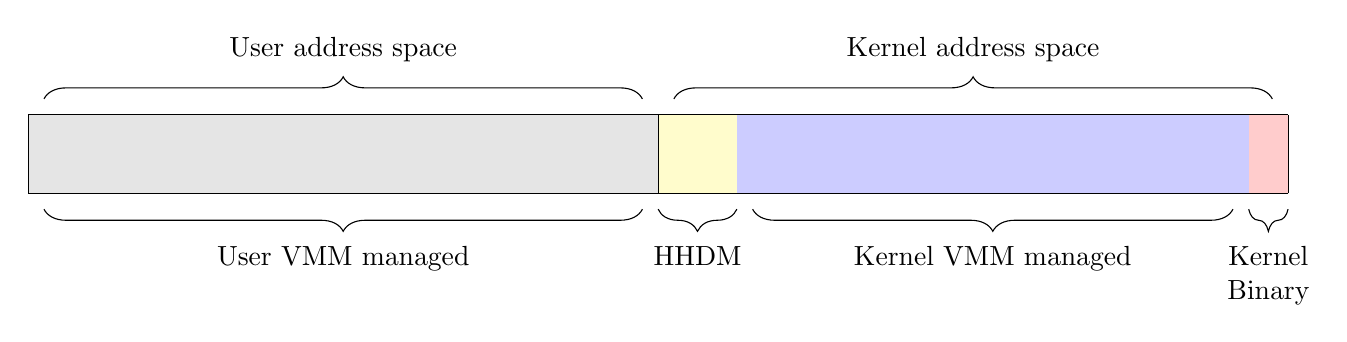
\begin{tikzpicture}
    \fill [gray!20] (0, 0) rectangle (8, 1);
    \fill [yellow!20] (8, 0) rectangle (9, 1);
    \fill [blue!20] (9, 0) rectangle (15.5, 1);
    \fill [red!20] (15.5, 0) rectangle (16, 1);

    \draw (0, 0) -- (16, 0);
    \draw (0, 1) -- (16, 1);
    \draw (0, 0) -- (0, 1);
    \draw (16, 0) -- (16, 1);
    \draw (8, 0) -- (8, 1);

    \draw[decoration={brace, amplitude=8pt},decorate] (0.2, 1.2) -- node[above=10pt] {User address space} (7.8, 1.2);
    \draw[decoration={brace, amplitude=8pt},decorate] (8.2, 1.2) -- node[above=10pt] {Kernel address space} (15.8, 1.2);
    \draw[decoration={brace, amplitude=8pt, mirror},decorate] (8, -0.2) -- node[below=10pt] {HHDM} (9, -0.2);
    \draw[decoration={brace, amplitude=8pt, mirror},decorate] (9.2, -0.2) -- node[below=10pt] {Kernel VMM managed} (15.3, -0.2);
    \draw[decoration={brace, amplitude=8pt, mirror},decorate] (15.5, -0.2) -- node[below=10pt,align=center] {Kernel\\Binary} (16, -0.2);
    \draw[decoration={brace, amplitude=8pt, mirror},decorate] (0.2, -0.2) -- node[below=10pt] {User VMM managed} (7.8, -0.2);
\end{tikzpicture}
\caption{Global address space layout.}
\end{figure}

\subsection{Meta Allocators}
Allocating memory for the VM ranges and address space hole structs can't be done via the global kernel heap, as the heap is built on top of virtual memory. To avoid this circular dependency, a VMM also contains a number of slab allocators known as \textit{meta allocators}. Each slab is sized around one type of metadata struct that needs to be stored: one slab for VM ranges, one for VM holes. Internally these allocators are quite simple, consisting of a linked list of individual slabs accompanied by a bitmap tracking a slab's free/in-use status.

The backing memory for these slabs are allocated directly from the PMM, and then these are accessed via the HHDM. This means the memory used for these allocators is managed outside the heap and virtual memory stacks and don't gain the benefits afforded by either of them (e.g. demand paging or CoW).

\subsection{Initialization}
Immediately after the physical memory manager is initialized, the kernel VMM is brought up. First \verb|HatInit()| is called, which allows the architecture layer to perform some global setup, as well as map the HHDM in the map used by the kernel VMM. The reason the HAT is responsible for mapping the HHDM instead of the VMM is that the HAT can freely make assumptions about the best way to map the large, continuous area of address that the HHDM occupies. This function is only called once and is therefore not suitable for core-local setup of the MMU. It's mainly for detecting what mode the MMU is in (e.g. how many paging levels are available and in use), and any optional extensions. Next the VM drivers are initialized, this mainly consists of detecting and setting some software feature flags. The exception here is the kernel VMM which maps the kernel binary with (proper permissions) into the address space of the kernel VMM.

It should be noted that at this point the kernel is still running using the MMU settings setup by the bootloader. The next step is the actually initialize the kernel VMM instance by telling it what range of addresses it has available: these start immediately after the HHDM and end just before the kernel binary begins. At this point the kernel VMM loads its own address map.

\subsection{Allocation}
There's a few key steps to allocating a new chunk of virttual memory. First the VMM finds the correct VM driver for the type of memory requested via the \verb|flags| argument. Then the VMM calls \verb|vmdriver.Query()| to determine exactly how much space is needed for the allocation and the required alignment. The VM driver might require more space for the allocation than was requested depending on the limits exposed by the HAT. For example if mapping a file via the VFS VM driver with an offset of 123 bytes, which is not aligned with the HAT mode chosen by the file cache. The VM driver would need to start mapping the VM range at the nearest address aligned to the chosen HAT mode, and then return a pointer 123 bytes beyond the start of the mapping.

\begin{figure}[h]
\centering
\caption{Example usage of the VM range offset field when mapping a file.}
\end{figure}

This mechanism of returning an offset into the allocated VM range also easily allows for other mechanisms like guard pages.

\begin{figure}[h]
\centering
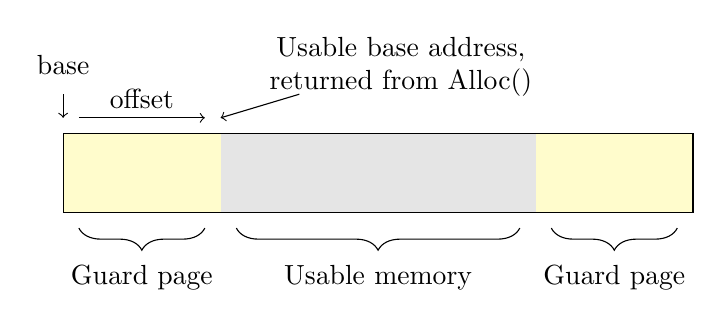
\begin{tikzpicture}
    \fill [yellow!20] (0, 0) rectangle (8, 1);
    \fill [gray!20] (2, 0) rectangle (6, 1);
    \draw (0, 0) rectangle (8, 1);

    \draw [->] (0, 1.5) -- node [above=8pt] {base} (0, 1.2);
    \draw [->] (0.2, 1.2) -- node [above] {offset} (1.8, 1.2);
    \draw [->] (3, 1.5) -- node [above right,align=center] {Usable base address,\\returned from Alloc()} (2, 1.2);

    \draw[decoration={brace, amplitude=8pt, mirror},decorate] (0.2, -0.2) --node [below=10pt] {Guard page} (1.8, -0.2);
    \draw[decoration={brace, amplitude=8pt, mirror},decorate] (2.2, -0.2) --node [below=10pt] {Usable memory} (5.8, -0.2);
    \draw[decoration={brace, amplitude=8pt, mirror},decorate] (6.2, -0.2) --node [below=10pt] {Guard page} (7.8, -0.2);
\end{tikzpicture}
\caption{Using the offset field for Guard Pages.}
\end{figure}

After calling \verb|Query()| on the VM driver, the VMM finds an appropriate area of unused address space for the VM range to occupy, and creates a new VM range struct. The free space is marked as in-use and the VM range struct is populated with details like the base address and length of the range.

At this point the VMM calls \verb|vmdriver.Attach()| which is where the VM driver begins managing the mappings associated with the VM range. Note that the driver isn't required to actually map anything yet, depending on it's configuration. It may wait for the VMM to signal a fault before committing any physical memory or other resources. During this function the VM driver can return a \textit{token}, which acts as a private pointer between the range and the VM driver. This token is stored in the VM range struct, and is available to the driver any time it's requested to oeprate on the VM range.

Once the VM driver is attached, the range is inserted in the \verb|ranges| tree and is now considered active.

\subsection{Usage of Page Faults}
The VMM and VM drivers make full usage of page faults (and handling them). Often a fault is triggered by the hardware in response to action taken by a program, but a page fault can also be triggered manually by calling \verb|HandleFault()| on any VMM to trigger the same response. This function returns a bool indicating if the fault was considered 'good' or not. A good fault is an allowed (and expected) memory access, while a bad fault is an illegal one.

Bad faults can result in any number of consequences, from a program being terminated to a kernel panic, depending on the VMM in question.

When handling a page fault the VMM will check the faulting address against the list of active VM ranges, looking for the associated range. If a matching range isn't found, the fault returns \verb|false| as it failed to handle it properly. If the range is found, the VMM will then check the fault flags which describe what the memory access was (read, write or execute), it's privilege level (supervisor or user). Assuming the memory access was allowed for this VM range, the VMM will call the fault handler on the VM driver attached to the range and allow the driver to continue handling the fault. At this point the VM driver is responsible for the outcome of the fault.

VM drivers may choose to not map physical memory with the full permissions requested by the VMM, in order to trigger a fault on certain actions. This is used to implement features like CoW (copy-on-write), zero-paging, or to allow the backing memory to be reclaimed and used elsewhere. \textit{Currently swapping to disk isn't implemented, and the file cache is only half transient - it has no page-out features}

At this point the action taken depends on the specific VM driver and the exact nature of the fault.

\subsection{Example Code}
Allocating and freeing can be done by calling the VMM directly, or by using a VMO. The kernel VMM is accessible through a static function \lstinline{VMM::Kernel()} and the active user VMM can be access similarly as \lstinline{VMM::Current()}. The VMM and associated structs are declared in \verb|memory/Vmm.h|, to use VMOs without including the rest of the virtual memory related code you can just include |verb|memory/VmObject.h|.

The \lstinline{Alloc()} function accepts a size and flags argument. The flags contains permissions (write and execute, all memory is readable), the type of memory required (MMIO, anon or file-backed) and some other flags for adjusting the behaviour of this VM range. There is also an \lstinline{initArg} argument, the purpose of which depends on the type of memory requested: for MMIO it's the base physical address of the MMIO to map, for anonymous memory it's a set of feature flags to disable for this allocation, and for for-backed memory it contains a pointer to a \lstinline{VmoFileInitArg}.

As an example we'll allocate 123 bytes of writable anonymous virtual memory in kernel address space, and then free it.
\begin{lstlisting}
sl::Opt<uintptr_t> maybeMem = VMM::Kernel().Alloc(
    123, 0, VmFlag::Anon | VmFlag::Write);

//Note that Alloc() returns an Opt<>, meaning allocation can fail!
uintptr_t vaddr = *maybeMem;
//Not required, but Free() returns if it was successful or not
ASSERT(VMM::Kernel().Free(vaddr), "VMM::Free()");
\end{lstlisting}

Mapping MMIO is equally straightfoward, we can pass the physical address we want to map to the \lstinline{initArg}.
\begin{lstlisting}
uintptr_t mmioBase = 0xFEE00000;
auto mem = VMM::Kernel().Alloc(0x1000, mmioBase, VmFlags::Mmio);
ASSERT(mem.HasValue(), "VMM::Alloc()");
\end{lstlisting}

In the previous example we mapped the MMIO as readonly, as we didn't specify the write flag. Lets say this was intentional, and we only wanted it to be writable later on. It's possible to try modify the flags of an active range, although the attached VM driver may refuse the new flags. It's also currently not possible to change the type of virtual memory by just changing the flags, and trying this will result in the operation simply failing. This example continues on from the previous one, and will attempt to make the MMIO writable.
\begin{lstlisting}
if (VMM::Kernel().SetFlags(*mem, VmFlags::Write))
    Log("Made MMIO writable", LogLevel::Debug);
\end{lstlisting}

Finally for allocation, let's look at using file-backed memory. Backing virtual memory with the contents of the file cache is done by setting \lstinline{VmFlag::File} and passing a pointer to a \lstinline{VmoFileInfoArg} as the \verb|initArg|. For this example we're going to map a file called \verb|/somedir/example.txt|, and we want our view of the file to start 42 bytes into the file and be 0x1000 bytes long.

\begin{lstlisting}
VmoFileInitArg initArg {};
initArg.filepath = "/somedir/example.txt";
initArg.offset = 42;

VmFlags flags = VmFlag::File | VmFlag::Write;
auto mem = VMM::Kernel().Alloc(0x1000, &initArg, flags);
ASSERT(mem.HasValue(), "Memory mapping file failed.");
\end{lstlisting}

The VMM also provides some utility functions for copying data in and out of an address space, relative to the currently active one. These functions are not needed for the kernel VMM as it's always active, but if accessing data in a user VMM that is not the active one, they allow for this. These functions act similarly to the standard \lstinline{memcopy()}.

There is also a function for getting the physical address of a backed virtual one.
\begin{lstlisting}
uintptr_t vaddr;
sl::Opt<uintptr_t> maybePhys = VMM::Kernel().GetPhysical(vaddr);

if (maybePhys.HasValue())
    Log("virt=0x%lx, phys=0x%lx", LogLevel::Debug, vaddr, *maybePhys);
else
    Log("No translation for 0x%lx", LogLevel::Debug, vaddr);
\end{lstlisting}
